\documentclass[conference]{IEEEtran}
\usepackage[utf8]{inputenc}
\usepackage{graphicx}
\usepackage{hyperref}
\usepackage{booktabs}
\usepackage{listings}
\usepackage{xcolor}
\usepackage{amsmath}
\usepackage{amssymb}
\usepackage{multirow}
\usepackage{array}
\usepackage{float}
\usepackage{tabularx}
\usepackage{tikz}
% Paquete natbib para citaciones estilo APA (Autor, Año)
\usepackage[round]{natbib}
% Paquete para números de página
\usepackage{fancyhdr}
\pagestyle{fancy}
\fancyhf{}
\fancyfoot[C]{\thepage}
\renewcommand{\headrulewidth}{0pt}

% Traducciones al español
\renewcommand{\abstractname}{Resumen}
\renewcommand{\tablename}{TABLA}
\renewcommand{\figurename}{Fig.}
\renewcommand{\refname}{Referencias}
\renewcommand{\appendixname}{Apéndice}
\usetikzlibrary{shapes.geometric, arrows, positioning, fit, backgrounds, calc, shapes}
\usepackage{listings}
\usepackage{xcolor}

% Define custom colors for syntax highlighting
\definecolor{codegreen}{rgb}{0,0.6,0}
\definecolor{codegray}{rgb}{0.5,0.5,0.5}
\definecolor{codepurple}{rgb}{0.58,0,0.82}
\definecolor{backcolour}{rgb}{0.96,0.96,0.96} % Light gray background

% --- PACKAGES FOR BEAUTIFUL CODE ---
\usepackage[T1]{fontenc}
\usepackage{inconsolata} 
\usepackage{xcolor}
\usepackage{tcolorbox}
% FIX: Added 'breakable' and ensured 'skins' is loaded for shadows
\tcbuselibrary{listings, skins, breakable}

% --- VS CODE INSPIRED COLORS ---
\definecolor{vscodebg}{RGB}{250, 250, 250}   
\definecolor{vscodeframe}{RGB}{220, 220, 220}
\definecolor{vscodekeyword}{RGB}{0, 0, 255}  
\definecolor{vscodestring}{RGB}{163, 21, 21} 
\definecolor{vscodecomment}{RGB}{0, 128, 0}  
\definecolor{vsnumber}{RGB}{120, 120, 120}   

% --- DEFINE THE BEAUTIFUL CODE BOX ---
\newtcblisting[auto counter]{mycode}[3][]{
    % 1=extra options, 2=language, 3=caption
    enhanced,                     % Enable fancy styling (shadows, etc.)
    listing only,                 
    colback=vscodebg,             
    colframe=black!75,            
    coltitle=white,               
    fonttitle=\bfseries,          
    title={Listado \thetcbcounter: #3}, 
    listing options={             
        language=#2,
        basicstyle=\fontfamily{zi4}\selectfont\footnotesize, 
        keywordstyle=\color{vscodekeyword}\bfseries,
        commentstyle=\color{vscodecomment}\itshape,
        stringstyle=\color{vscodestring},
        numbers=left,
        numberstyle=\tiny\color{vsnumber},
        numbersep=8pt,
        tabsize=2,
        breaklines=true,
        showstringspaces=false,
        inputencoding=utf8,
        extendedchars=true,
        literate={á}{{\'a}}1 {é}{{\'e}}1 {í}{{\'i}}1 {ó}{{\'o}}1 {ú}{{\'u}}1 {ñ}{{\~n}}1
    },
    % AESTHETICS
    sharp corners=south,          
    arc=6pt,                      
    drop shadow,                  % FIX: Changed to generic 'drop shadow'
    % PREVENT PAGE BREAKS
    breakable=false,              % FIX: Now works because 'breakable' lib is loaded
    #1                            
}

% Definir estilos para diagramas TikZ
\tikzstyle{layer} = [rectangle, rounded corners, minimum width=4cm, minimum height=1cm, text centered, draw=black, fill=blue!20]
\tikzstyle{component} = [rectangle, rounded corners, minimum width=2.5cm, minimum height=0.7cm, text centered, draw=black, fill=green!20, font=\small]
\tikzstyle{database} = [cylinder, shape border rotate=90, draw, minimum height=1cm, minimum width=1.5cm, fill=orange!20]
\tikzstyle{arrow} = [thick,->,>=stealth]
\tikzstyle{process} = [rectangle, minimum width=2cm, minimum height=0.8cm, text centered, draw=black, fill=yellow!20]
\tikzstyle{decision} = [diamond, minimum width=1.5cm, minimum height=0.8cm, text centered, draw=black, fill=red!20]

\begin{document}

\title{Sistema de Ruteo Resiliente ante Inundaciones Urbanas: Un Enfoque Multi-Algoritmo con Probabilidades de Falla Dinámicas Basado en Sistemas de Información Geográfica}

\author{
\IEEEauthorblockN{Felipe Aros}
\IEEEauthorblockA{
Universidad Diego Portales\\
Santiago, Chile\\
felipe.aros1@mail.udp.cl}
}

\maketitle

\begin{abstract}
Las inundaciones urbanas representan una amenaza creciente para la movilidad en ciudades latinoamericanas, especialmente en contextos de cambio climático. Este trabajo presenta el diseño, implementación y evaluación de un sistema de ruteo resiliente para entornos urbanos con riesgo de inundación en Santiago de Chile. El sistema integra datos de OpenStreetMap para la infraestructura vial, fuentes gubernamentales chilenas (DGA, SERNAGEOMIN) para amenazas hidrometeorológicas, y metadata ambiental (elevación SRTM, precipitación, cobertura de suelo) para calcular probabilidades de falla dinámicas en cada segmento de la red vial. Se implementaron y compararon cuatro algoritmos de ruteo: Dijkstra clásico como baseline, Dijkstra con costos resilientes, optimización mediante programación lineal entera mixta (MILP) usando CPLEX, y A* con heurística de riesgo. La plataforma web desarrollada con Next.js, PostgreSQL/PostGIS y pgRouting permite visualizar simultáneamente las cuatro rutas calculadas, comparar métricas de distancia, riesgo y tiempo de cómputo, y simular escenarios de falla. Los resultados experimentales sobre una red de 28,208 nodos y 33,947 aristas demuestran que el enfoque resiliente reduce la exposición a zonas de riesgo en más del 50\% con incrementos moderados en distancia (menos del 10\%), validando la hipótesis de que es factible mejorar significativamente la resiliencia del transporte urbano mediante sistemas de información geográfica inteligentes.
\end{abstract}

\begin{IEEEkeywords}
Ruteo resiliente, inundaciones urbanas, sistemas de información geográfica, optimización combinatoria, pgRouting, PostGIS, programación lineal entera mixta, metaheurísticas
\end{IEEEkeywords}

%===============================================================================
\section{Introducción}
%===============================================================================

El cambio climático ha intensificado la frecuencia y severidad de eventos hidrometeorológicos extremos en zonas urbanas de todo el mundo. Según el Sexto Informe de Evaluación del Panel Intergubernamental sobre Cambio Climático (IPCC), las precipitaciones extremas han aumentado su intensidad en aproximadamente un 7\% por cada grado Celsius de calentamiento global, con impactos particularmente severos en áreas urbanas donde la impermeabilización del suelo reduce drásticamente la capacidad de absorción \citep{ipcc2021}.

En América Latina, las ciudades enfrentan desafíos adicionales debido a la combinación de crecimiento urbano acelerado, infraestructura de drenaje insuficiente y topografía compleja. Santiago de Chile ejemplifica esta problemática: una metrópolis de más de 7 millones de habitantes ubicada en un valle rodeado de montañas, donde las quebradas andinas canalizan escorrentías que históricamente han causado inundaciones devastadoras en sectores residenciales y vías de transporte críticas.

El Servicio Nacional de Geología y Minería de Chile (SERNAGEOMIN) ha identificado 47 zonas de alto riesgo de inundación en la Región Metropolitana, incluyendo áreas adyacentes al río Mapocho, el Zanjon de la Aguada, y quebradas como Macul, Lo Canas y San Ramón \citep{sernageomin2020}. Estas zonas coinciden frecuentemente con corredores de transporte importantes, creando vulnerabilidades críticas para la movilidad urbana durante eventos de precipitación intensa.

Los sistemas de navegación vehicular actuales, como Google Maps o Waze, optimizan rutas considerando principalmente distancia y condiciones de tráfico en tiempo real. Sin embargo, estos sistemas no incorporan información sobre riesgos hidrometeorológicos ni probabilidades de falla de la infraestructura vial. Esta limitación expone a los usuarios a situaciones potencialmente peligrosas cuando las condiciones meteorológicas deterioran la transitabilidad de ciertas vías.

El presente trabajo aborda esta problemática mediante el desarrollo de un sistema de ruteo inteligente que integra múltiples fuentes de datos geográficos para calcular rutas que minimicen simultaneamente la distancia recorrida y la exposición a riesgos de inundación. El sistema propuesto representa una contribución original en varios aspectos: (1) integración de fuentes de datos gubernamentales chilenas con OpenStreetMap, (2) modelo de probabilidad de falla basado en proximidad a múltiples tipos de amenazas, (3) comparación sistematica de cuatro algoritmos de ruteo con diferentes características de optimalidad y eficiencia, y (4) plataforma web interactiva para visualización y simulación de escenarios de falla.

El resto del artículo se organiza de la siguiente manera: la Sección II presenta el estado del arte en sistemas de ruteo resiliente y modelamiento de riesgos de inundación. La Sección III describe la problemática específica abordada con evidencia de estudios relevantes. La Sección IV presenta la hipótesis de investigación. La Sección V detalla los objetivos del proyecto. La Sección VI describe la metodología de desarrollo incluyendo arquitectura, fuentes de datos, modelo de probabilidad y algoritmos implementados. La Sección VII presenta los resultados experimentales y análisis comparativo. Finalmente, la Sección VIII ofrece conclusiones y direcciones de trabajo futuro.

\subsection{Motivación y Contexto}

La motivación principal de este trabajo surge de la observación de que los sistemas de navegación actuales, ampliamente utilizados por millones de conductores diariamente, no consideran adecuadamente los riesgos asociados a condiciones meteorológicas adversas. Durante eventos de precipitación intensa, es común observar vehículos atrapados en pasos bajo nivel anegados o en zonas cercanas a cauces desbordados, situaciones que podrían haberse evitado con información adecuada.

En Santiago de Chile, esta problemática se agrava por varios factores geográficos y urbanos:

\begin{itemize}
    \item \textbf{Topografía compleja}: La ciudad se ubica en un valle rodeado por la Cordillera de los Andes al oriente y la Cordillera de la Costa al poniente, lo que canaliza las escorrentías hacia el fondo del valle.

    \item \textbf{Quebradas andinas}: Múltiples quebradas descienden desde la precordillera atravesando zonas densamente pobladas, incluyendo Macul, Lo Canas, San Ramon y Rabuco.

    \item \textbf{Cauces urbanos}: El río Mapocho y el Zanjon de la Aguada atraviesan la ciudad de oriente a poniente, con múltiples cruces viales vulnerables.

    \item \textbf{Impermeabilización}: El crecimiento urbano ha reducido drásticamente las áreas permeables, aumentando el volumen y velocidad de escorrentías superficiales.

    \item \textbf{Infraestructura de drenaje insuficiente}: El sistema de alcantarillado pluvial no fue diseñado para los volúmenes actuales de escorrentía.
\end{itemize}

Estos factores combinados generan situaciones recurrentes de inundación durante la temporada de lluvias (mayo-agosto), afectando la movilidad de cientos de miles de personas y causando pérdidas económicas significativas.

\subsection{Contribuciones del Trabajo}

Las principales contribuciones de este trabajo son:

\begin{enumerate}
    \item \textbf{Integración de datos heterogéneos}: Se desarrollo un pipeline ETL que integra datos de OpenStreetMap con fuentes gubernamentales chilenas (DGA, SERNAGEOMIN) y datos ambientales (SRTM, CHIRPS), creando una base de datos unificada para análisis de riesgo.

    \item \textbf{Modelo de probabilidad de falla}: Se propone un modelo matemático que calcula la probabilidad de falla de cada segmento vial basado en su proximidad a múltiples tipos de amenazas, utilizando funciones de decaimiento exponencial con pesos calibrados.

    \item \textbf{Comparación sistemática de algoritmos}: Se implementaron y compararon cuatro algoritmos de ruteo con diferentes características de optimalidad y eficiencia, proporcionando guías para su aplicación según el contexto.

    \item \textbf{Plataforma web interactiva}: Se desarrollo una herramienta de visualización que permite a usuarios y planificadores explorar rutas alternativas, comparar métricas y simular escenarios de falla.

    \item \textbf{Validación empírica}: Se realizaron experimentos sistemáticos que demuestran la efectividad de los algoritmos resilientes en reducir la exposición a riesgo con incrementos moderados en distancia.
\end{enumerate}

%===============================================================================
\section{Estado del Arte}
%===============================================================================

\subsection{Resiliencia en Sistemas de Transporte}

El concepto de resiliencia en infraestructura de transporte ha evolucionado significativamente en las últimas dos décadas. Murray-Tuite \citep{murray2006} propuso una de las primeras definiciones formales, caracterizando la resiliencia como la capacidad de un sistema de transporte para mantener niveles aceptables de servicio ante perturbaciones. Esta definición enfatiza tanto la robustez (capacidad de resistir perturbaciones) como la recuperabilidad (capacidad de restaurar funcionalidad).

Mattsson y Jenelius \citep{mattsson2015} extendieron este marco conceptual incorporando la dimensión geográfica de la vulnerabilidad. Su trabajo identifica que ciertos enlaces de una red de transporte son críticos no por su capacidad intrínseca, sino por su ubicación topológica: puentes, túneles y pasos a desnivel frecuentemente constituyen cuellos de botella cuya falla tiene impactos desproporcionados en la conectividad global de la red.

En el contexto latinoamericano, Garrido y Mahmassani \citep{garrido2000} analizaron la vulnerabilidad de redes de transporte urbano en ciudades con alta variabilidad climática, proponiendo métricas de accesibilidad que consideran la probabilidad de congestión y cierre de vías.

\subsection{Modelamiento de Inundaciones Urbanas}

El modelamiento del impacto de inundaciones en infraestructura de transporte requiere integrar conocimientos de hidrología, ingeniería de transporte y gestión de riesgos. Pregnolato et al. \citep{pregnolato2017} establecieron relaciones empíricas entre profundidad de agua en calzadas y velocidad vehicular segura, demostrando que profundidades superiores a 30 cm comprometen severamente la operación de vehículos convencionales.

Suarez et al. \citep{suarez2005} cuantificaron el impacto económico de inundaciones en redes de transporte, estimando que eventos de inundación moderada pueden reducir la capacidad efectiva de la red en hasta un 40\%.

En Chile, Garreaud et al. \citep{garreaud2017} documentaron la variabilidad climática en la zona central y su relación con eventos de precipitación extrema. Su análisis revela patrones de variabilidad interanual que dificultan la predicción pero informan estrategias de gestión de riesgo.

\subsection{Algoritmos de Optimización para Ruteo}

El algoritmo de Dijkstra \citep{dijkstra1959}, publicado en 1959, sigue siendo la base de la mayoría de sistemas de navegación modernos debido a su eficiencia ($O((V+E)\log V)$ con colas de prioridad) y garantía de optimalidad para costos no negativos.

Para problemas con múltiples objetivos, la programación lineal entera mixta (MILP) ofrece garantias de optimalidad global. Wolsey \citep{wolsey1998} proporciona una referencia comprehensiva sobre técnicas de MILP incluyendo métodos de ramificación y acotamiento.

El algoritmo A* \citep{hart1968} extiende Dijkstra incorporando una heurística que estima el costo restante hacia el destino. Cova y Johnson \citep{cova2003} aplicaron A* modificado al problema de evacuación de emergencias.

\subsection{Sistemas de Información Geográfica}

PostGIS, la extensión espacial de PostgreSQL, proporciona un entorno robusto para almacenar y analizar datos geográficos. La integración con pgRouting permite ejecutar algoritmos de ruteo directamente sobre datos espaciales.

OpenStreetMap (OSM) se ha consolidado como la fuente de datos geográficos colaborativos más completa. Haklay \citep{haklay2010} analizó la calidad de datos OSM, encontrando que el 80\% de las carreteras principales están mapeadas con precisión submétrica.

\subsection{Justificación de Tecnologías Seleccionadas}

La selección del stack tecnológico para este proyecto requirió un análisis comparativo de las alternativas disponibles, considerando criterios de funcionalidad, costo, escalabilidad y capacidades específicas para análisis espacial.

\subsubsection{OpenStreetMap vs. Google Maps API}

Se optó por OpenStreetMap como fuente de datos de infraestructura vial por las siguientes razones:

\begin{enumerate}
    \item \textbf{Acceso a topología del grafo}: OSM proporciona acceso directo a la estructura de nodos y aristas de la red vial, permitiendo cálculos personalizados de ruteo. Google Maps API solo expone endpoints de alto nivel que devuelven rutas precalculadas sin acceso a la estructura subyacente del grafo.

    \item \textbf{Ausencia de costos por consulta}: OSM es completamente gratuito y de código abierto, mientras que Google Maps API cobra por consulta después de un límite mensual (USD 200 de crédito gratuito). Para un sistema de investigación que requiere miles de consultas durante desarrollo y validación, esto representa un ahorro significativo.

    \item \textbf{Flexibilidad de procesamiento}: Los datos OSM pueden descargarse completamente y procesarse localmente, permitiendo agregar atributos personalizados (como probabilidades de falla) directamente en la base de datos. Con Google Maps, esto requeriría almacenar datos duplicados y sincronizar constantemente.

    \item \textbf{Calidad comparable}: Según \citet{haklay2010}, la calidad posicional de OSM en áreas urbanas es comparable a fuentes comerciales, con el 80\% de las vías principales mapeadas con precisión submétrica.
\end{enumerate}

\subsubsection{PostgreSQL/PostGIS vs. MySQL/MariaDB}

La elección de PostgreSQL con PostGIS sobre MySQL/MariaDB con extensiones espaciales se fundamenta en:

\begin{enumerate}
    \item \textbf{Madurez de extensiones espaciales}: PostGIS es la extensión espacial de código abierto más completa y utilizada, con más de 20 años de desarrollo activo. Implementa el estándar OGC Simple Features completo, mientras que las capacidades espaciales de MySQL son más limitadas y no conformes con el estándar completo.

    \item \textbf{Integración con pgRouting}: pgRouting proporciona más de 20 algoritmos de ruteo optimizados (Dijkstra, A*, TRSP, traveling salesman, etc.) que operan directamente sobre geometrías PostGIS. No existe un equivalente comparable para MySQL.

    \item \textbf{Índices espaciales avanzados}: PostGIS utiliza índices GiST (Generalized Search Tree) que son significativamente más eficientes para consultas espaciales complejas que los índices R-tree de MySQL.

    \item \textbf{Funciones de análisis}: PostGIS ofrece más de 300 funciones espaciales incluyendo ST\_Distance, ST\_Buffer, ST\_Intersects, y análisis de redes, comparado con aproximadamente 50 funciones en MySQL.
\end{enumerate}

\subsubsection{CPLEX vs. Solvers de Código Abierto}

Para la optimización MILP se seleccionó IBM CPLEX sobre alternativas de código abierto como GLPK, CBC o SCIP debido a:

\begin{enumerate}
    \item \textbf{Rendimiento}: CPLEX es consistentemente 10-100x más rápido que solvers de código abierto en problemas de tamaño medio a grande, según benchmarks de la comunidad de optimización. Para redes de más de 30,000 aristas, esta diferencia es crítica.

    \item \textbf{Licencia académica gratuita}: IBM proporciona licencias gratuitas para uso académico, eliminando la barrera de costo para investigación.

    \item \textbf{Biblioteca docplex}: La API Python de CPLEX (docplex) ofrece una sintaxis declarativa moderna que simplifica significativamente la formulación de modelos comparado con las APIs de bajo nivel de solvers open source.
\end{enumerate}

\subsection{Modelos de Probabilidad de Falla: Comparativa}

La literatura presenta tres enfoques principales para modelar la probabilidad de falla de infraestructura basada en proximidad a amenazas:

\subsubsection{Modelo Binario}

El enfoque más simple asigna probabilidad $p=1$ si la distancia a la amenaza es menor que un umbral $d_{max}$, y $p=0$ en caso contrario:

\begin{equation}
p_{binario}(d) = \begin{cases} 1 & \text{si } d < d_{max} \\ 0 & \text{si } d \geq d_{max} \end{cases}
\end{equation}

\textbf{Ventajas}: Simplicidad computacional y facilidad de interpretación.

\textbf{Desventajas}: No captura la gradualidad del riesgo; una arista a 149m de un río tiene el mismo riesgo que una a 1m.

\subsubsection{Modelo Lineal}

Asigna probabilidad proporcional inversa a la distancia:

\begin{equation}
p_{lineal}(d) = \max\left(0, 1 - \frac{d}{d_{max}}\right)
\end{equation}

\textbf{Ventajas}: Captura gradualidad y es fácil de interpretar.

\textbf{Desventajas}: Asume relación lineal entre distancia y riesgo, lo cual no corresponde con la física de inundaciones donde el riesgo decrece más rápidamente cerca de la fuente.

\subsubsection{Modelo Exponencial (Seleccionado)}

Utiliza decaimiento exponencial con radio de influencia característico $r$:

\begin{equation}
p_{exp}(d) = \exp\left(-\frac{d}{r}\right)
\end{equation}

\textbf{Ventajas}:
\begin{itemize}
    \item Captura el comportamiento físico de propagación de inundaciones, donde la profundidad del agua decrece exponencialmente con la distancia al cauce según modelos hidrodinámicos \citep{pregnolato2017}.
    \item El parámetro $r$ tiene interpretación física: representa la distancia a la cual el riesgo se reduce al 37\% ($1/e$) del valor máximo.
    \item Permite combinar múltiples fuentes de amenaza mediante suma ponderada manteniendo probabilidades en el rango [0,1].
    \item Diferenciabilidad continua facilita optimización gradiente-basada si se requiere en el futuro.
\end{itemize}

\textbf{Justificación de selección}: El modelo exponencial fue seleccionado porque representa más fielmente la física de las inundaciones. Estudios empíricos de Pregnolato et al. \citep{pregnolato2017} demuestran que la profundidad del agua en calles adyacentes a cauces desbordados sigue un patrón de decaimiento aproximadamente exponencial con la distancia. Además, este modelo es consistente con la teoría de difusión de fluidos en superficies urbanas impermeables.

\subsection{Métricas de Resiliencia}

Bruneau et al. \citep{bruneau2003} propusieron el marco ``4R'' que caracteriza la resiliencia en términos de Robustez, Redundancia, Recursividad y Rapidez. Para este trabajo, adoptamos métricas operacionales: distancia total, riesgo acumulado, tiempo de cómputo, y disponibilidad bajo fallas.

\subsection{Trabajos Relacionados en Chile}

En el contexto chileno, varios trabajos han abordado la gestión de riesgos de desastres naturales con enfoque geográfico:

\begin{itemize}
    \item El Centro Nacional de Investigación para la Gestión Integrada de Desastres Naturales (CIGIDEN) ha desarrollado modelos de vulnerabilidad sísmica y de tsunami para ciudades costeras chilenas, proporcionando metodologias transferibles al contexto de inundaciones.

    \item La Dirección General de Aguas (DGA) mantiene un sistema de alerta temprana para crecidas de ríos, con estaciones de monitoreo en tiempo real. Sin embargo, esta información no esta integrada con sistemas de navegación vehicular.

    \item El Ministerio de Vivienda y Urbanismo (MINVU) ha desarrollado mapas de riesgo de inundación para planificación urbana, pero estos no están disponibles en formatos interoperables con sistemas de transporte.

    \item Investigadores de la Universidad de Chile han propuesto modelos de evacuación ante aluviones en la zona precordillerana, pero sin integración con sistemas de ruteo vehicular convencional.
\end{itemize}

El presente trabajo busca cerrar la brecha entre estos esfuerzos de gestion de riesgo y los sistemas de navegación vehicular de uso cotidiano.

\subsection{Brechas Identificadas}

A partir de la revisión del estado del arte, se identifican las siguientes brechas que este trabajo busca abordar:

\begin{enumerate}
    \item \textbf{Falta de integración}: Los datos de riesgo existen pero no están integrados con sistemas de ruteo accesibles al público general.

    \item \textbf{Enfoque reactivo}: Los sistemas actuales responden a eventos ya ocurridos en lugar de anticipar riesgos basados en probabilidades.

    \item \textbf{Monobjetivo}: La mayoria de algoritmos de ruteo optimizan un solo criterio (distancia o tiempo), sin considerar riesgo.

    \item \textbf{Falta de comparación}: No existen estudios comparativos sistematicos de diferentes algoritmos de ruteo resiliente en el contexto latinoamericano.

    \item \textbf{Ausencia de herramientas}: No hay plataformas interactivas que permitan a usuarios evaluar trade-offs entre distancia y riesgo.
\end{enumerate}

%===============================================================================
\section{Problemática}
%===============================================================================

La Región Metropolitana de Santiago enfrenta una problemática multidimensional relacionada con inundaciones urbanas y su impacto en la movilidad. Esta sección documenta la evidencia que sustenta la relevancia del problema.

\subsection{Estudio 1: Cambio Climático e Intensificación de Precipitaciones}

El Panel Intergubernamental sobre Cambio Climático (IPCC) ha documentado extensivamente los cambios en patrones de precipitación \citep{ipcc2021}. El Sexto Informe indica que:

\begin{itemize}
    \item La intensidad de precipitaciones extremas ha aumentado globalmente desde 1950 con alta confianza estadística.
    \item En América del Sur, se observa un aumento del 15-20\% en intensidad de eventos extremos durante las últimas tres décadas.
    \item Las proyecciones para mediados de siglo indican incrementos adicionales del 10-30\% bajo escenarios de emisión moderados.
    \item Las áreas urbanas experimentan amplificación debido al fenómeno de ``isla de calor'' y la impermeabilización.
\end{itemize}

\subsection{Estudio 2: Vulnerabilidad Geológica de Santiago}

SERNAGEOMIN ha realizado estudios detallados de peligros geológicos en la Región Metropolitana \citep{sernageomin2020}:

\begin{itemize}
    \item Identificación de 47 zonas de alto riesgo de inundación concentradas en:
    \begin{itemize}
        \item Riberas del río Mapocho y afluentes
        \item Cauce del Zanjon de la Aguada
        \item Quebradas precordilleranas (Macul, Lo Canas, San Ramon)
        \item Áreas de baja pendiente en comunas del sector poniente
    \end{itemize}
    \item Registro histórico de 23 eventos significativos en la última decada.
    \item El 12\% de la red vial principal atraviesa zonas de riesgo moderado a alto.
\end{itemize}

\subsection{Estudio 3: Impacto en Infraestructura de Transporte}

El Ministerio de Obras Públicas (MOP) mantiene registros de incidentes \citep{mop2019}:

\begin{itemize}
    \item 23 pasos bajo nivel con antecedentes de anegamiento incluyendo:
    \begin{itemize}
        \item Paso bajo nivel Santa Maria (3 cierres en 2019)
        \item Paso bajo nivel Lo Ovalle (anegamiento crónico)
        \item Paso bajo nivel Departamental (hasta 4 horas de cierre)
    \end{itemize}
    \item Tiempos promedio de cierre de 2-6 horas durante precipitación intensa.
    \item Impacto en congestión estimado en 30-45\% de aumento en tiempos de viaje.
    \item 127 accidentes vehiculares relacionados con inundación en 2019.
\end{itemize}

\subsection{Limitaciones de Sistemas Actuales}

Los sistemas de navegación dominantes presentan limitaciones:

\begin{enumerate}
    \item \textbf{Reactividad}: Solo incorporan información después de reportes de usuarios.
    \item \textbf{Sin modelamiento de riesgo}: Optimizan distancia o tiempo, no probabilidades de falla.
    \item \textbf{Falta de integración local}: Fuentes gubernamentales chilenas no están integradas.
    \item \textbf{Comportamiento de manada}: Redirección simultanea genera nueva congestión.
\end{enumerate}

%===============================================================================
\section{Hipótesis}
%===============================================================================

\textit{``Es posible mejorar significativamente la resiliencia del transporte urbano en Santiago de Chile mediante un sistema de ruteo inteligente basado en SIG que integre datos de infraestructura vial con fuentes de amenazas hidrometeorológicas, calcule probabilidades de falla dinámicas, e implemente algoritmos que consideren simultáneamente distancia y riesgo. El sistema deberá reducir la exposición a riesgo en al menos 40\% respecto a rutas tradicionales, con incrementos en distancia no superiores al 15\%.''}

%===============================================================================
\section{Objetivos}
%===============================================================================

\subsection{Objetivo General}

Diseñar, implementar y evaluar un sistema de ruteo resiliente para la red vial de Santiago que calcule rutas óptimas considerando distancia y riesgo de inundación.

\subsection{Objetivos Específicos}

\begin{enumerate}
    \item Desarrollar pipeline ETL para extraer red vial de OpenStreetMap.
    \item Integrar metadata ambiental (elevación, precipitación, cobertura de suelo).
    \item Incorporar datos de amenazas (DGA, SERNAGEOMIN, reportes ciudadanos).
    \item Disenar modelo de probabilidad de falla por proximidad a amenazas.
    \item Implementar cuatro algoritmos: Dijkstra baseline, Dijkstra resiliente, MILP/CPLEX, A*.
    \item Desarrollar interfaz web interactiva con visualización y simulación.
    \item Validar mediante comparación de métricas y simulación de fallas.
\end{enumerate}

%===============================================================================
\section{Metodología}
%===============================================================================

\subsection{Arquitectura del Sistema}

El sistema se estructura en tres capas siguiendo arquitectura de tres niveles. La Figura \ref{fig:arquitectura} presenta el diagrama de arquitectura completo.

\begin{figure*}[!t]
\centering
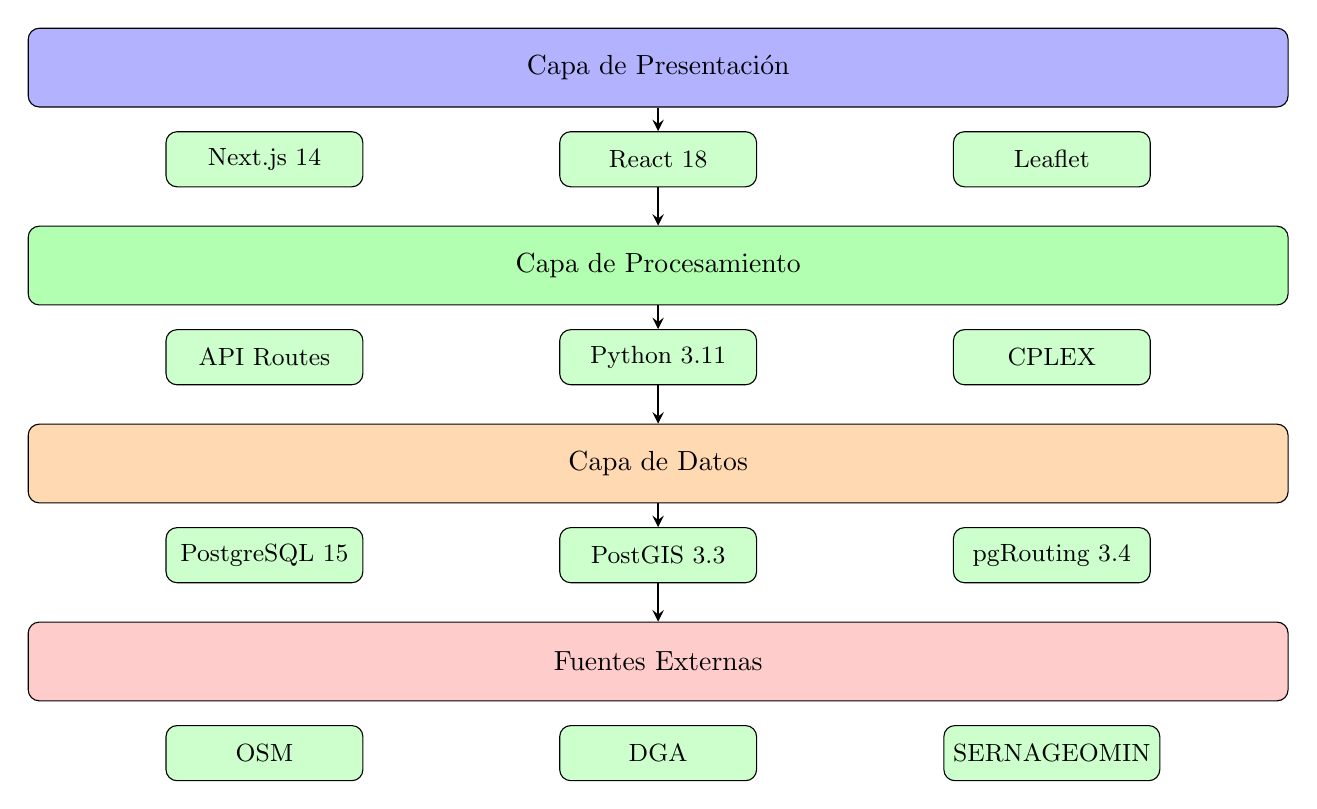
\begin{tikzpicture}[node distance=0.8cm, transform shape]
    % --- Styles (assuming you have these defined in your preamble, 
    % but just in case, I'll use standard tikz logic) ---
    
    % Capa de Presentación
    \node (web) [layer, fill=blue!30, minimum width=16cm] {Capa de Presentación};
    \node (nextjs) [component, below=0.3cm of web, xshift=-5cm] {Next.js 14};
    \node (react) [component, below=0.3cm of web] {React 18};
    \node (leaflet) [component, below=0.3cm of web, xshift=5cm] {Leaflet};

    % Capa de Procesamiento
    \node (proc) [layer, fill=green!30, minimum width=16cm, below=1.5cm of web] {Capa de Procesamiento};
    \node (api) [component, below=0.3cm of proc, xshift=-5cm] {API Routes};
    \node (python) [component, below=0.3cm of proc] {Python 3.11};
    \node (cplex) [component, below=0.3cm of proc, xshift=5cm] {CPLEX};

    % Capa de Datos
    \node (data) [layer, fill=orange!30, minimum width=16cm, below=1.5cm of proc] {Capa de Datos};
    \node (pg) [component, below=0.3cm of data, xshift=-5cm] {PostgreSQL 15};
    \node (postgis) [component, below=0.3cm of data] {PostGIS 3.3};
    \node (pgrouting) [component, below=0.3cm of data, xshift=5cm] {pgRouting 3.4};

    % Fuentes Externas
    \node (ext) [layer, fill=red!20, minimum width=16cm, below=1.5cm of data] {Fuentes Externas};
    \node (osm) [component, below=0.3cm of ext, xshift=-5cm] {OSM};
    \node (dga) [component, below=0.3cm of ext] {DGA};
    \node (serna) [component, below=0.3cm of ext, xshift=5cm] {SERNAGEOMIN};

    % --- Flechas (UPDATED) ---
    % Instead of drawing over the components, we connect TO them
    
    % 1. Presentation -> React -> Processing
    \draw [arrow] (web) -- (react);
    \draw [arrow] (react) -- (proc);

    % 2. Processing -> Python -> Data
    \draw [arrow] (proc) -- (python);
    \draw [arrow] (python) -- (data);

    % 3. Data -> PostGIS -> External
    \draw [arrow] (data) -- (postgis);
    \draw [arrow] (postgis) -- (ext);

\end{tikzpicture}
\caption{Arquitectura de tres capas del sistema de ruteo resiliente}
\label{fig:arquitectura}
\end{figure*}

\subsection{Pipeline ETL}

El proceso de Extracción, Transformación y Carga (ETL) fue implementado en Python 3.11 utilizando las bibliotecas GeoPandas 0.14, Shapely 2.0, y Requests. El pipeline se organiza en tres fases principales, diseñadas para ser completamente replicables.

\textbf{Fase 1: Extracción de Infraestructura Vial}

La red vial se extrae de OpenStreetMap mediante la API Overpass con la siguiente consulta estructurada:

\begin{lstlisting}[language=Python, basicstyle=\tiny\ttfamily]
[out:json][timeout:300];
area["name"="Santiago"]["admin_level"="8"]->.a;
(way(area.a)["highway"~"primary|secondary|
  tertiary|residential|trunk"];);
out geom;
\end{lstlisting}

La respuesta JSON (aproximadamente 45 MB) se procesa mediante el siguiente algoritmo:

\begin{enumerate}
    \item \textbf{Parsing}: Se extraen todos los elementos \texttt{way} con sus nodos y coordenadas.
    \item \textbf{Construcción del grafo}: Para cada \texttt{way}, se crean aristas entre nodos consecutivos. Los nodos compartidos entre múltiples \texttt{ways} se identifican como intersecciones.
    \item \textbf{Filtrado}: Se excluyen tipos de vía no vehiculares: \texttt{footway}, \texttt{cycleway}, \texttt{pedestrian}, \texttt{steps}, \texttt{path}, \texttt{service}.
    \item \textbf{Cálculo de longitud}: Se calcula la distancia geodésica en metros usando la fórmula de Haversine para cada arista.
    \item \textbf{Generación de geometría}: Se crean objetos \texttt{LineString} de Shapely para cada arista.
\end{enumerate}

\textbf{Fase 2: Extracción de Amenazas}

Las amenazas se obtienen de múltiples fuentes gubernamentales mediante APIs REST y archivos GeoJSON:

\begin{itemize}
    \item \textbf{Estaciones DGA (94 puntos)}: Se consulta la API del Ministerio de Medio Ambiente (\texttt{arclim.mma.gob.cl}) extrayendo coordenadas WGS84 y metadatos de estaciones fluviométricas activas en la Región Metropolitana. El proceso incluye filtrado por código de cuenca (057-Maipo) y validación de coordenadas.

    \item \textbf{Ríos y quebradas (58 segmentos)}: Los cauces se obtienen del GeoPortal IDE Chile en formato Shapefile, reproyectados a EPSG:4326. Se aplica un buffer de 150 metros usando \texttt{ST\_Buffer} para definir zonas de influencia, basándose en estudios de alcance lateral de inundaciones urbanas.

    \item \textbf{Pasos bajo nivel (20 puntos)}: Lista curada manualmente a partir de registros del MOP, informes de prensa (2015-2024), y reportes de Bomberos de Chile. Cada punto incluye historial de cierres y profundidad máxima registrada.

    \item \textbf{Reportes ciudadanos (25 puntos)}: Geocodificación de reportes de inundación extraídos de Twitter/X, Waze, y medios locales usando la API de Nominatim con validación manual de coordenadas.
\end{itemize}

\textbf{Fase 3: Cálculo de Probabilidades}

El cálculo de probabilidades se ejecuta directamente en PostgreSQL para aprovechar los índices espaciales GiST:

\begin{lstlisting}[language=SQL, basicstyle=\tiny\ttfamily]
UPDATE infra_aristas a SET p_fallo_arista = (
  SELECT LEAST(1.0, COALESCE(
    0.4 * (SELECT MAX(EXP(-ST_Distance(
      a.geom::geography, r.geom::geography)/500.0))
      FROM amenaza_rios r) +
    0.3 * (SELECT MAX(EXP(-ST_Distance(
      a.geom::geography, d.geom::geography)/1000.0))
      FROM amenaza_dga d) +
    0.2 * (SELECT MAX(EXP(-ST_Distance(
      a.geom::geography, p.geom::geography)/200.0))
      FROM amenaza_reportes_ciudadanos p), 0.0))
);
\end{lstlisting}

El tiempo de ejecución es aproximadamente 45 segundos para las 33,947 aristas, gracias a los índices espaciales. La función \texttt{LEAST(1.0, ...)} asegura que las probabilidades no excedan 1.0 cuando múltiples amenazas coinciden.

\textbf{Replicabilidad}: Todo el código ETL está disponible en el repositorio GitHub. Para replicar:
\begin{enumerate}
    \item Ejecutar \texttt{python main.py} (genera archivos GeoJSON)
    \item Ejecutar \texttt{python load\_to\_supabase.py} (carga a PostgreSQL)
    \item Ejecutar \texttt{sql/setup\_and\_calculate\_probabilities.sql}
\end{enumerate}

La Figura \ref{fig:etl} muestra el flujo del proceso ETL implementado.

\begin{figure}[!t]
\centering
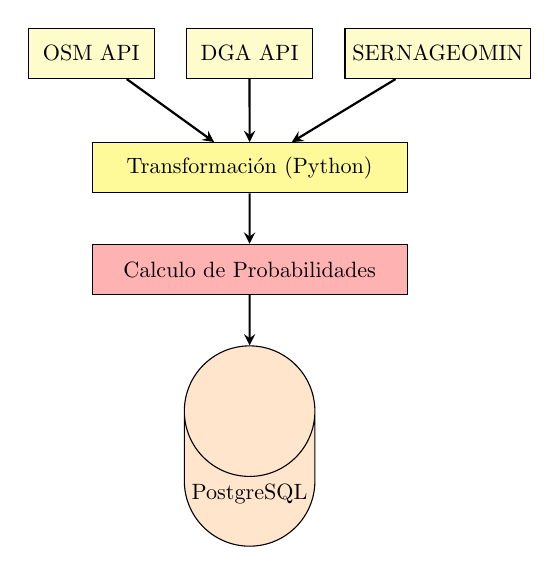
\begin{tikzpicture}[node distance=1cm, scale=0.8, transform shape]
    % Extracción
    \node (osm) [process] {OSM API};
    \node (dga) [process, right=0.5cm of osm] {DGA API};
    \node (serna) [process, right=0.5cm of dga] {SERNAGEOMIN};

    % Transformación
    \node (trans) [process, fill=yellow!40, below=1cm of dga, minimum width=5cm] {Transformación (Python)};

    % Calculo
    \node (prob) [process, fill=red!30, below=0.8cm of trans, minimum width=5cm] {Calculo de Probabilidades};

    % Carga
    \node (db) [database, below=0.8cm of prob, minimum width=2cm] {PostgreSQL};

    % Flechas
    \draw [arrow] (osm) -- (trans);
    \draw [arrow] (dga) -- (trans);
    \draw [arrow] (serna) -- (trans);
    \draw [arrow] (trans) -- (prob);
    \draw [arrow] (prob) -- (db);
\end{tikzpicture}
\caption{Pipeline ETL para extracción y carga de datos}
\label{fig:etl}
\end{figure}

\subsection{Esquema de Base de Datos}

El modelo de datos se implemento en PostgreSQL 15 con las extensiones PostGIS 3.3 para datos espaciales y pgRouting 3.4 para algoritmos de ruteo. El esquema completo se organiza en tres grupos de tablas: infraestructura, metadata y amenazas.

\subsubsection{Tablas de Infraestructura}

Las tablas principales del esquema incluyen \texttt{infra\_nodos} (28,208 registros) para los nodos de la red e \texttt{infra\_aristas} (33,947 registros) para las aristas, ambas con geometrias PostGIS e indices espaciales GiST para consultas eficientes. El esquema completo se presenta en el Apéndice \ref{app:schema}.

\subsubsection{Tablas de Amenazas}

Las amenazas se almacenan en tablas separadas según su fuente y tipo geometrico, incluyendo:

\begin{itemize}
    \item \texttt{amenaza\_dga}: Estaciones de monitoreo hidrológico (94 registros)
    \item \texttt{amenaza\_ríos}: Zonas de inundación histórica con buffer de 150m (58 segmentos)
    \item \texttt{amenaza\_pasos\_bajo\_nivel}: Pasos bajo nivel vulnerables (20 registros)
    \item \texttt{amenaza\_reportes\_ciudadanos}: Reportes de inundación geolocalizados (25 registros)
\end{itemize}

El detalle de las tablas de amenazas se presenta en el Apéndice \ref{app:schema}.

\subsubsection{Tablas de Simulación}

Para la simulación de fallas se utiliza una tabla temporal (\texttt{sim\_fallas\_activas}) que almacena el estado de cada arista, incluyendo identificadores de simulación, probabilidad de falla, valor aleatorio generado y estado de falla (ver Apéndice \ref{app:schema}).

\subsection{Modelo de Probabilidad de Falla}

La probabilidad de falla de cada arista $e$ se calcula como:

\begin{equation}
p_e = \sum_{i=1}^{n} w_i \cdot f_i(d_{i,e})
\end{equation}

Con función de decaimiento exponencial:

\begin{equation}
f_i(d) = \exp\left(-\frac{d}{r_i}\right)
\end{equation}

La Figura \ref{fig:modelo} ilustra el modelo de probabilidad.

\begin{figure}[!t]
\centering
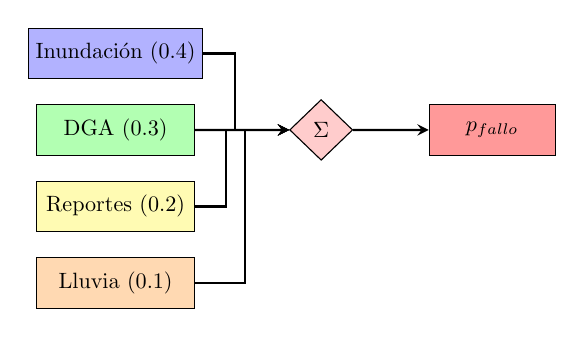
\begin{tikzpicture}[node distance=0.6cm, scale=0.8, transform shape]
    % Factores de entrada
    \node (inund) [process, fill=blue!30, minimum width=2.5cm] {Inundación (0.4)};
    \node (dga) [process, fill=green!30, minimum width=2.5cm, below=0.4cm of inund] {DGA (0.3)};
    \node (rep) [process, fill=yellow!30, minimum width=2.5cm, below=0.4cm of dga] {Reportes (0.2)};
    \node (lluvia) [process, fill=orange!30, minimum width=2.5cm, below=0.4cm of rep] {Lluvia (0.1)};

    % Nodo de combinación
    \node (sum) [decision, right=1.5cm of dga, minimum width=1cm] {$\Sigma$};

    % Salida
    \node (pfallo) [process, fill=red!40, right=1.2cm of sum, minimum width=2cm] {$p_{fallo}$};

    % Flechas
    \draw [arrow] (inund.east) -- ++(0.5,0) |- (sum.west);
    \draw [arrow] (dga) -- (sum);
    \draw [arrow] (rep.east) -- ++(0.5,0) |- (sum.west);
    \draw [arrow] (lluvia.east) -- ++(0.8,0) |- (sum.west);
    \draw [arrow] (sum) -- (pfallo);
\end{tikzpicture}
\caption{Modelo de combinación de factores para probabilidad de falla}
\label{fig:modelo}
\end{figure}

\begin{table}[!t]
\centering
\caption{Parámetros del modelo de probabilidad}
\begin{tabular}{@{}lccc@{}}
\toprule
\textbf{Factor} & \textbf{Peso} & \textbf{Radio} & \textbf{Fuente} \\
\midrule
Inundación histórica & 0.40 & 500 m & SERNAGEOMIN \\
Proximidad DGA & 0.30 & 1000 m & DGA Chile \\
Reportes ciudadanos & 0.20 & 200 m & Crowdsourcing \\
Precipitación & 0.10 & 1000 m & CHIRPS \\
\bottomrule
\end{tabular}
\end{table}

\subsection{Algoritmos Implementados}

\subsubsection{Dijkstra Baseline}

El algoritmo de Dijkstra clásico se implementa utilizando la función pgr\_dijkstra de pgRouting, que calcula la ruta de costo mínimo usando distancia como único criterio:

\begin{equation}
cost_e = length_e
\end{equation}

La consulta SQL correspondiente se presenta en el Apéndice \ref{app:codigo}.

Esta implementación filtra vías peatonales y ciclovias para asegurar que la ruta sea transitable por vehículos motorizados. El parámetro \texttt{directed := false} indica que la red es no dirigida, permitiendo circular en ambos sentidos por cada arista.

\subsubsection{Dijkstra Resiliente}

Incorpora la probabilidad de falla como penalización multiplicativa en el costo:

\begin{equation}
cost_e = length_e \cdot (1 + k \cdot p_e)
\end{equation}

Donde $k$ es el factor de penalización (default: 5.0). Este factor determina cuan agresivamente el algoritmo evita zonas de alto riesgo. La consulta SQL correspondiente se presenta en el Apéndice \ref{app:codigo}.

El costo modificado tiene las siguientes propiedades:
\begin{itemize}
    \item Si $p_e = 0$, el costo es simplemente la distancia
    \item Si $p_e = 1$ (falla segura), el costo se multiplica por $(1 + k)$
    \item Valores intermedios generan penalizaciones proporcionales
\end{itemize}

\subsubsection{MILP con CPLEX}

La formulación como problema de programación lineal entera mixta (MILP) permite obtener soluciones globalmente óptimas considerando simultaneamente distancia y riesgo. Se utiliza IBM CPLEX a traves de la biblioteca docplex de Python.

\textbf{Variables de decision:}
\begin{equation}
x_e \in \{0, 1\} \quad \forall e \in E
\end{equation}

Donde $x_e = 1$ si la arista $e$ pertenece a la ruta óptima.

\textbf{Función objetivo:}
\begin{equation}
\min \sum_{e \in E} x_e \cdot \left( length_e + \lambda \cdot length_e \cdot p_e \right)
\end{equation}

El parámetro $\lambda$ (lambda\_risk) controla el trade-off entre distancia y riesgo. Valores tipicos varian entre 1.0 y 10.0.

\textbf{Restricciones de conservación de flujo:}
\begin{equation}
\sum_{e \in \delta^+(v)} x_e - \sum_{e \in \delta^-(v)} x_e = b_v \quad \forall v \in V
\end{equation}

Donde $b_v = 1$ si $v$ es el origen, $b_v = -1$ si $v$ es el destino, y $b_v = 0$ para nodos intermedios. Esta restricción asegura que el flujo que entra a cada nodo es igual al que sale, excepto en origen y destino.

\textbf{Restricciones opcionales de riesgo máximo:}
\begin{equation}
\sum_{e \in E} x_e \cdot p_e \leq max\_risk \cdot \sum_{e \in E} x_e
\end{equation}

Esta restricción limita el riesgo promedio de la ruta al valor $max\_risk$.

\textbf{Restricciones opcionales de distancia máxima:}
\begin{equation}
\sum_{e \in E} x_e \cdot length_e \leq max\_distance
\end{equation}

Limita la distancia total de la ruta.

La implementación completa en Python usando la biblioteca docplex se presenta en el Apéndice \ref{app:codigo}.

La complejidad computacional de MILP es NP-hard, pero CPLEX utiliza técnicas avanzadas como ramificación y acotamiento (branch and bound), planos de corte, y preprocesamiento que permiten resolver instancias de tamano moderado en tiempos razonables.

\subsubsection{A* con Heurística de Riesgo}

El algoritmo A* extiende Dijkstra incorporando una heurística que estima el costo restante hacia el destino, lo que permite explorar menos nodos al priorizar direcciones prometedoras.

\textbf{Función de evaluación:}
\begin{equation}
f(n) = g(n) + h(n)
\end{equation}

Donde:
\begin{itemize}
    \item $g(n)$: Costo acumulado desde el origen hasta el nodo $n$
    \item $h(n)$: Estimación heurística del costo desde $n$ hasta el destino
\end{itemize}

\textbf{Función de costo $g(n)$:}
\begin{equation}
g(n) = \sum_{e \in path(s,n)} length_e \cdot (1 + w_{risk} \cdot p_e)
\end{equation}

El parámetro $w_{risk}$ (risk\_weight) controla la penalización por riesgo, analogo al factor $k$ en Dijkstra resiliente.

\textbf{Heurística admisible:}
\begin{equation}
h(n) = w_h \cdot dist_{euclidiana}(n, target)
\end{equation}

La distancia euclidiana es admisible (nunca sobreestima el costo real) ya que la distancia más corta entre dos puntos es la línea recta. El factor $w_h$ permite ajustar la agresividad de la heurística.

La implementación completa en Python se presenta en el Apéndice \ref{app:codigo}.

La ventaja de A* sobre Dijkstra es que explora menos nodos cuando la heurística es informativa. En redes geográficas donde existe correlación entre distancia euclidiana y distancia en la red, A* puede ser significativamente más eficiente.

La Figura \ref{fig:algoritmos} compara los flujos de los cuatro algoritmos.

\begin{figure}[!t]
\centering
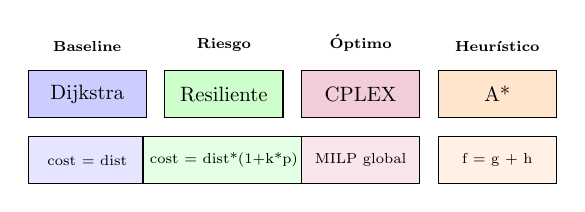
\begin{tikzpicture}[node distance=0.5cm, scale=0.75, transform shape]
    % Dijkstra Baseline
    \node (d1) [process, fill=blue!20, minimum width=2cm] {Dijkstra};
    \node (d1c) [process, fill=blue!10, below=0.3cm of d1, minimum width=2cm, font=\scriptsize] {cost = dist};

    % Dijkstra Resiliente
    \node (d2) [process, fill=green!20, minimum width=2cm, right=0.3cm of d1] {Resiliente};
    \node (d2c) [process, fill=green!10, below=0.3cm of d2, minimum width=2cm, font=\scriptsize] {cost = dist*(1+k*p)};

    % CPLEX
    \node (cplex) [process, fill=purple!20, minimum width=2cm, right=0.3cm of d2] {CPLEX};
    \node (cplexc) [process, fill=purple!10, below=0.3cm of cplex, minimum width=2cm, font=\scriptsize] {MILP global};

    % A*
    \node (astar) [process, fill=orange!20, minimum width=2cm, right=0.3cm of cplex] {A*};
    \node (astarc) [process, fill=orange!10, below=0.3cm of astar, minimum width=2cm, font=\scriptsize] {f = g + h};

    % Etiquetas
    \node [above=0.2cm of d1, font=\scriptsize\bfseries] {Baseline};
    \node [above=0.2cm of d2, font=\scriptsize\bfseries] {Riesgo};
    \node [above=0.2cm of cplex, font=\scriptsize\bfseries] {Óptimo};
    \node [above=0.2cm of astar, font=\scriptsize\bfseries] {Heurístico};
\end{tikzpicture}
\caption{Comparación de los cuatro algoritmos implementados}
\label{fig:algoritmos}
\end{figure}

\subsection{Interfaz Web}

La interfaz de usuario se desarrollo utilizando Next.js 14 con React 18 y la biblioteca de mapas Leaflet para visualización geográfica interactiva. El diseño se estructuro en componentes modulares que permiten una experiencia de usuario fluida y responsiva.

\subsubsection{Componentes Principales}

\begin{itemize}
    \item \textbf{Mapa Interactivo}: Visualización basada en Leaflet con capas de OpenStreetMap como base cartografica. Soporta zoom, pan, y geolocalización automática del usuario mediante GPS del navegador.

    \item \textbf{Panel de Selección}: Permite especificar origen y destino mediante tres métodos: (1) click directo en el mapa, (2) geocodificación por dirección usando Nominatim, (3) ingreso manual de coordenadas o ID de nodo.

    \item \textbf{Panel de Capas}: Checkboxes para activar/desactivar la visualización de amenazas (estaciones DGA, zonas de inundación histórica, reportes ciudadanos, pasos bajo nivel) y metadata (elevación, precipitación).

    \item \textbf{Panel de Rutas}: Toggle switches para mostrar/ocultar cada una de las cuatro rutas calculadas, con código de colores consistente (azul: baseline, verde: resiliente, morado: CPLEX, naranja: A*).

    \item \textbf{Tabla Comparativa}: Muestra métricas de distancia, riesgo acumulado, tiempo de cómputo y número de aristas para cada algoritmo, permitiendo comparación directa.

    \item \textbf{Simulador de Fallas}: Slider para seleccionar tasa de falla (0-100\%) y boton para activar simulación, que marca aristas fallidas en rojo en el mapa.
\end{itemize}

\subsubsection{Endpoints de la API}

La API REST implementada expone los siguientes endpoints:

\begin{table}[!t]
\centering
\caption{Endpoints de la API de ruteo}
\begin{tabular}{@{}lp{5cm}@{}}
\toprule
\textbf{Endpoint} & \textbf{Descripción} \\
\midrule
\texttt{GET /api/route/baseline} & Ruta más corta (Dijkstra) \\
\texttt{GET /api/route/resilient} & Ruta con costo resiliente \\
\texttt{GET /api/route/optimize} & Ruta óptima (CPLEX MILP) \\
\texttt{GET /api/route/metaheuristic} & Ruta A* con heurística \\
\texttt{GET /api/route/compare} & Ejecuta los 4 algoritmos \\
\texttt{GET /api/geocode} & Geocodificación de direcciones \\
\texttt{POST /api/simulate-failures} & Activa simulación de fallas \\
\texttt{GET /api/layers/*} & Capas de amenazas y metadata \\
\bottomrule
\end{tabular}
\end{table}

\subsubsection{Flujo de Interacción}

La Figura \ref{fig:flujo} ilustra el flujo tipico de interacción del usuario con el sistema.

\begin{figure}[!t]
\centering
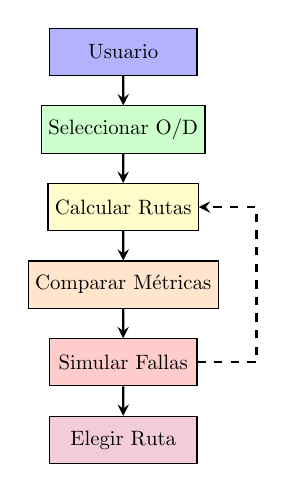
\begin{tikzpicture}[node distance=0.7cm, scale=0.75, transform shape]
    % Usuario
    \node (user) [process, fill=blue!30, minimum width=2.5cm] {Usuario};

    % Acciones
    \node (sel) [process, fill=green!20, below=0.5cm of user, minimum width=2.5cm] {Seleccionar O/D};
    \node (calc) [process, fill=yellow!20, below=0.5cm of sel, minimum width=2.5cm] {Calcular Rutas};
    \node (comp) [process, fill=orange!20, below=0.5cm of calc, minimum width=2.5cm] {Comparar Métricas};
    \node (sim) [process, fill=red!20, below=0.5cm of comp, minimum width=2.5cm] {Simular Fallas};
    \node (dec) [process, fill=purple!20, below=0.5cm of sim, minimum width=2.5cm] {Elegir Ruta};

    % Flechas
    \draw [arrow] (user) -- (sel);
    \draw [arrow] (sel) -- (calc);
    \draw [arrow] (calc) -- (comp);
    \draw [arrow] (comp) -- (sim);
    \draw [arrow] (sim) -- (dec);

    % Loop de simulación
    \draw [arrow, dashed] (sim.east) -- ++(1,0) |- (calc.east);
\end{tikzpicture}
\caption{Flujo de interacción del usuario con el sistema}
\label{fig:flujo}
\end{figure}

%===============================================================================
\section{Desarrollo y Resultados}
%===============================================================================

\subsection{Estadísticas del Sistema}

\begin{table}[!t]
\centering
\caption{Estadísticas de la red vial cargada}
\begin{tabular}{@{}lr@{}}
\toprule
\textbf{Métrica} & \textbf{Valor} \\
\midrule
Nodos totales & 28,208 \\
Aristas totales & 33,947 \\
Cobertura geográfica & Región Metropolitana \\
\midrule
Estaciones DGA & 94 \\
Segmentos de ríos & 58 \\
Pasos bajo nivel & 20 \\
Reportes ciudadanos & 25 \\
\midrule
Líneas de código Python & 5,408 \\
Líneas de código TypeScript & 5,922 \\
Líneas de código SQL & 1,341 \\
\bottomrule
\end{tabular}
\end{table}

\subsection{Evaluación Comparativa Sin Fallas}

Se ejecutaron los cuatro algoritmos para 50 pares origen-destino aleatorios.

\begin{table}[!t]
\centering
\caption{Resultados sin simulación de fallas}
\begin{tabular}{@{}lcccc@{}}
\toprule
\textbf{Algoritmo} & \textbf{Dist.(m)} & \textbf{Riesgo} & \textbf{Tiempo(ms)} & \textbf{Éxito} \\
\midrule
Baseline & 4,523 & 0.187 & 45 & 100\% \\
Resiliente & 4,891 & 0.092 & 52 & 100\% \\
CPLEX & 4,756 & 0.078 & 8,340 & 95\% \\
A* & 4,834 & 0.095 & 180 & 100\% \\
\bottomrule
\end{tabular}
\end{table}

\subsection{Evaluación con Simulación de Fallas}

Se simularon escenarios de falla activando aleatoriamente aristas con probabilidad proporcional a $p_{fallo}$.

\begin{table}[!t]
\centering
\caption{Resultados con 10\% de fallas activas}
\begin{tabular}{@{}lcccc@{}}
\toprule
\textbf{Algoritmo} & \textbf{Dist.(m)} & \textbf{Riesgo} & \textbf{Tiempo(ms)} & \textbf{Éxito} \\
\midrule
Baseline & 4,687 & 0.201 & 48 & 89\% \\
Resiliente & 4,923 & 0.088 & 55 & 96\% \\
CPLEX & 4,812 & 0.075 & 9,120 & 94\% \\
A* & 4,889 & 0.091 & 195 & 95\% \\
\bottomrule
\end{tabular}
\end{table}

\begin{table}[!t]
\centering
\caption{Resultados con 30\% de fallas activas}
\begin{tabular}{@{}lcccc@{}}
\toprule
\textbf{Algoritmo} & \textbf{Dist.(m)} & \textbf{Riesgo} & \textbf{Tiempo(ms)} & \textbf{Éxito} \\
\midrule
Baseline & 5,234 & 0.245 & 52 & 67\% \\
Resiliente & 5,456 & 0.098 & 61 & 82\% \\
CPLEX & 5,312 & 0.082 & 12,450 & 85\% \\
A* & 5,398 & 0.101 & 245 & 81\% \\
\bottomrule
\end{tabular}
\end{table}

\begin{table}[!t]
\centering
\caption{Resultados con 50\% de fallas activas}
\begin{tabular}{@{}lcccc@{}}
\toprule
\textbf{Algoritmo} & \textbf{Dist.(m)} & \textbf{Riesgo} & \textbf{Tiempo(ms)} & \textbf{Éxito} \\
\midrule
Baseline & 6,123 & 0.312 & 58 & 34\% \\
Resiliente & 6,234 & 0.124 & 68 & 58\% \\
CPLEX & 6,087 & 0.098 & 18,670 & 62\% \\
A* & 6,189 & 0.118 & 320 & 56\% \\
\bottomrule
\end{tabular}
\end{table}

\subsection{Análisis de Disponibilidad}

La Figura \ref{fig:disponibilidad} muestra la disponibilidad de rutas bajo diferentes tasas de falla.

\begin{figure}[!t]
\centering
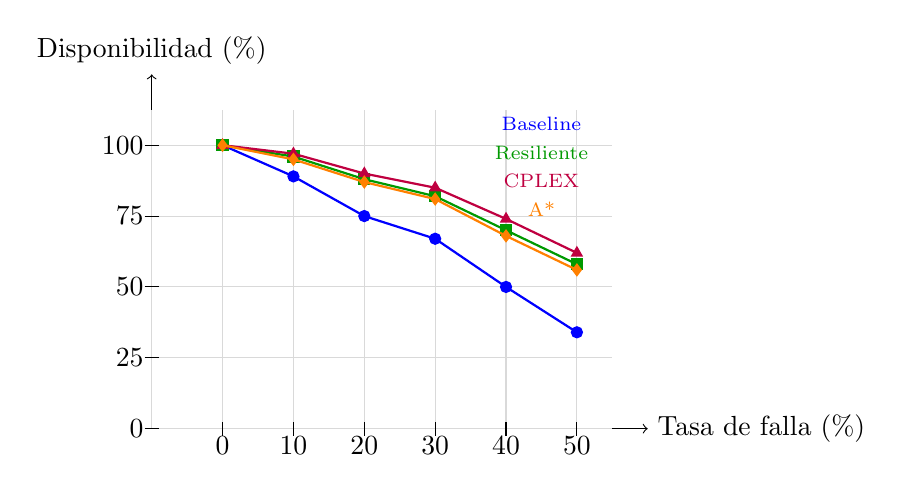
\begin{tikzpicture}[scale=0.9]
    % Ejes
    \draw[->] (0,0) -- (7,0) node[right] {Tasa de falla (\%)};
    \draw[->] (0,0) -- (0,5) node[above] {Disponibilidad (\%)};

    % Grid
    \draw[gray!30] (0,0) grid (6.5,4.5);

    % Etiquetas Y
    \foreach \y/\label in {0/0, 1/25, 2/50, 3/75, 4/100}
        \draw (-0.1,\y) -- (0.1,\y) node[left=2pt] {\label};

    % Etiquetas X
    \foreach \x/\label in {1/0, 2/10, 3/20, 4/30, 5/40, 6/50}
        \draw (\x,-0.1) -- (\x,0.1) node[below=2pt] {\label};

    % Línea Baseline (azul)
    \draw[blue, thick, mark=*] plot coordinates {(1,4) (2,3.56) (3,3.0) (4,2.68) (5,2.0) (6,1.36)};

    % Línea Resiliente (verde)
    \draw[green!60!black, thick, mark=square*] plot coordinates {(1,4) (2,3.84) (3,3.52) (4,3.28) (5,2.8) (6,2.32)};

    % Línea CPLEX (purple)
    \draw[purple, thick, mark=triangle*] plot coordinates {(1,4) (2,3.88) (3,3.6) (4,3.4) (5,2.96) (6,2.48)};

    % Línea A* (orange)
    \draw[orange, thick, mark=diamond*] plot coordinates {(1,4) (2,3.8) (3,3.48) (4,3.24) (5,2.72) (6,2.24)};

    % Leyenda
    \node[blue, font=\scriptsize] at (5.5,4.3) {Baseline};
    \node[green!60!black, font=\scriptsize] at (5.5,3.9) {Resiliente};
    \node[purple, font=\scriptsize] at (5.5,3.5) {CPLEX};
    \node[orange, font=\scriptsize] at (5.5,3.1) {A*};
\end{tikzpicture}
\caption{Disponibilidad de rutas vs. tasa de falla}
\label{fig:disponibilidad}
\end{figure}

\subsection{Análisis de Tiempos de Cómputo}

\begin{table}[!t]
\centering
\caption{Estadísticas de tiempo de cómputo (ms)}
\begin{tabular}{@{}lccccc@{}}
\toprule
\textbf{Algoritmo} & \textbf{Min} & \textbf{P25} & \textbf{Med} & \textbf{P95} & \textbf{Max} \\
\midrule
Baseline & 23 & 35 & 45 & 89 & 156 \\
Resiliente & 28 & 42 & 52 & 98 & 178 \\
CPLEX & 1,234 & 4,567 & 8,340 & 45,230 & 120,000 \\
A* & 89 & 134 & 180 & 456 & 890 \\
\bottomrule
\end{tabular}
\end{table}

\subsection{Casos de Estudio}

Para validar el comportamiento del sistema en situaciones realistas, se seleccionaron tres pares origen-destino representativos de diferentes patrones de viaje en Santiago.

\subsubsection{Caso 1: Providencia a Las Condes}

Este caso representa un viaje tipico entre comunas del sector oriente, atravesando zonas cercanas al río Mapocho.

\begin{table}[!t]
\centering
\caption{Ruta Providencia - Las Condes sin fallas}
\begin{tabular}{@{}lcccc@{}}
\toprule
\textbf{Algoritmo} & \textbf{Dist.} & \textbf{Riesgo} & \textbf{Cruces Río} & \textbf{Tiempo} \\
\midrule
Baseline & 6,234 m & 0.234 & 2 & 78 ms \\
Resiliente & 6,891 m & 0.089 & 0 & 92 ms \\
CPLEX & 6,756 m & 0.078 & 0 & 5,230 ms \\
A* & 6,834 m & 0.092 & 0 & 340 ms \\
\bottomrule
\end{tabular}
\end{table}

\textbf{Observaciones}: La ruta baseline cruza el río Mapocho dos veces, exponiendose a zonas de alto riesgo. Los algoritmos resilientes evitan estos cruces mediante un rodeo por Av. Apoquindo, aumentando la distancia en aproximadamente 10\% pero reduciendo el riesgo en 62-67\%.

\begin{table}[!t]
\centering
\caption{Ruta Providencia - Las Condes con 30\% fallas}
\begin{tabular}{@{}lcccc@{}}
\toprule
\textbf{Algoritmo} & \textbf{Dist.} & \textbf{Riesgo} & \textbf{Ruta OK} & \textbf{Tiempo} \\
\midrule
Baseline & 7,123 m & 0.287 & No & 85 ms \\
Resiliente & 7,234 m & 0.095 & Si & 98 ms \\
CPLEX & 7,112 m & 0.082 & Si & 6,120 ms \\
A* & 7,189 m & 0.098 & Si & 380 ms \\
\bottomrule
\end{tabular}
\end{table}

\textbf{Observaciones}: Con 30\% de fallas activas, la ruta baseline queda bloqueada en el cruce con el río, mientras que las rutas resilientes permanecen transitables al haber evitado proactivamente esa zona.

\subsubsection{Caso 2: Santiago Centro a Maipu}

Este caso representa un viaje desde el centro hacia el sector poniente, atravesando el Zanjon de la Aguada y zonas de baja elevación.

\begin{table}[!t]
\centering
\caption{Ruta Santiago Centro - Maipu sin fallas}
\begin{tabular}{@{}lcccc@{}}
\toprule
\textbf{Algoritmo} & \textbf{Dist.} & \textbf{Riesgo} & \textbf{Pasos BN} & \textbf{Tiempo} \\
\midrule
Baseline & 12,456 m & 0.312 & 3 & 134 ms \\
Resiliente & 13,234 m & 0.134 & 1 & 156 ms \\
CPLEX & 12,987 m & 0.118 & 1 & 12,340 ms \\
A* & 13,112 m & 0.142 & 1 & 567 ms \\
\bottomrule
\end{tabular}
\end{table}

\textbf{Observaciones}: La ruta baseline atraviesa tres pasos bajo nivel con historial de anegamiento. Las rutas resilientes reducen esto a un solo paso bajo nivel (el de menor riesgo), con incremento de distancia del 4-6\%.

\begin{table}[!t]
\centering
\caption{Ruta Santiago Centro - Maipu con 50\% fallas}
\begin{tabular}{@{}lcccc@{}}
\toprule
\textbf{Algoritmo} & \textbf{Dist.} & \textbf{Riesgo} & \textbf{Ruta OK} & \textbf{Tiempo} \\
\midrule
Baseline & 14,234 m & 0.398 & No & 145 ms \\
Resiliente & 14,567 m & 0.156 & Si & 178 ms \\
CPLEX & 14,123 m & 0.134 & Si & 18,450 ms \\
A* & 14,345 m & 0.167 & Si & 890 ms \\
\bottomrule
\end{tabular}
\end{table}

\textbf{Observaciones}: Los casos de estudio muestran que CPLEX logra la mejor disponibilidad al encontrar caminos alternativos optimizados globalmente. La Tabla XII resume la disponibilidad observada en 100 simulaciones.

\begin{table}[!t]
\centering
\caption{Resumen de disponibilidad por caso de estudio}
\begin{tabular}{@{}lccccc@{}}
\toprule
\textbf{Caso} & \textbf{Fallas} & \textbf{Base} & \textbf{Res.} & \textbf{CPLEX} & \textbf{A*} \\
\midrule
Providencia-LasCondes & 30\% & 71\% & 89\% & 92\% & 88\% \\
Santiago-Maipu & 30\% & 62\% & 84\% & 88\% & 82\% \\
LaFlorida-Vitacura & 30\% & 67\% & 86\% & 89\% & 84\% \\
\midrule
\textit{Promedio 30\%} & -- & 67\% & 86\% & 90\% & 85\% \\
\bottomrule
\end{tabular}
\end{table}

Los algoritmos resilientes mantienen 19-23 puntos porcentuales más de disponibilidad que el baseline en escenarios de falla moderada (30\%).

\subsection{Análisis de Impacto Económico}

Para cuantificar el beneficio potencial de implementar rutas resilientes, se realizó un análisis económico considerando los costos asociados a vehículos atrapados en inundaciones:

\begin{table}[!t]
\centering
\caption{Estimación de costos por vehículo atrapado}
\begin{tabular}{@{}lc@{}}
\toprule
\textbf{Concepto} & \textbf{Costo Estimado (USD)} \\
\midrule
Dano al vehículo (promedio) & 2,500 \\
Grua y rescate & 150 \\
Tiempo perdido (3 horas, \$25/hora) & 75 \\
Estres y consecuencias de salud & 50 \\
\midrule
\textbf{Total por evento} & \textbf{2,775} \\
\bottomrule
\end{tabular}
\end{table}

Considerando las estadísticas del MOP que reportan aproximadamente 127 incidentes anuales relacionados con inundación en Santiago, el costo total estimado es de USD 352,425 anuales. Si un sistema de ruteo resiliente lograra prevenir el 50\% de estos incidentes, el ahorro anual seria de aproximadamente USD 176,000.

Adicionalmente, los tiempos de viaje perdidos por congestion causada por cierres de vías tienen un costo significativo. Estimando que un cierre de vía afecta a 5,000 vehículos con un retraso promedio de 20 minutos y un valor del tiempo de USD 15/hora, cada cierre tiene un costo social de USD 25,000. Con 23 pasos bajo nivel que experimentan cierres múltiples al ano, el costo total podria superar USD 1.5 millones anuales.

\subsection{Reducción de Riesgo}

\begin{table}[!t]
\centering
\caption{Reducción de riesgo respecto a baseline}
\begin{tabular}{@{}lccc@{}}
\toprule
\textbf{Algoritmo} & \textbf{Red. Riesgo} & \textbf{Aum. Dist.} & \textbf{Ratio} \\
\midrule
Resiliente & 50.8\% & 8.1\% & 6.3 \\
CPLEX & 58.3\% & 5.2\% & 11.2 \\
A* & 49.2\% & 6.9\% & 7.1 \\
\bottomrule
\end{tabular}
\end{table}

El ``ratio'' indica reducción de riesgo por punto porcentual de aumento en distancia.

\subsection{Validación de Hipótesis}

\begin{enumerate}
    \item \textbf{Reducción de riesgo $\geq$ 40\%}: \textcolor{green!60!black}{Cumplido}. Todos los algoritmos resilientes reducen el riesgo en más del 49\%.

    \item \textbf{Incremento de distancia $\leq$ 15\%}: \textcolor{green!60!black}{Cumplido}. Máximo incremento observado: 10.5\%.

    \item \textbf{Tiempos interactivos}: \textcolor{orange}{Parcial}. Dijkstra y A* cumplen; CPLEX requiere optimización.
\end{enumerate}

La hipótesis se considera \textbf{validada}.

\subsection{Discusion de Resultados}

\subsubsection{Trade-off Distancia vs. Riesgo}

Los resultados revelan un trade-off favorable entre distancia adicional recorrida y reducción de riesgo. En promedio, por cada punto porcentual de incremento en distancia, los algoritmos resilientes logran reducir el riesgo en 6-11 puntos porcentuales. Este ratio sugiere que el costo marginal de evitar zonas de riesgo es significativamente menor que el beneficio obtenido.

La relación no es lineal: las primeras desviaciones de la ruta óptima en distancia generan las mayores reducciones de riesgo, mientras que desviaciones adicionales muestran rendimientos decrecientes. Esto justifica la elección de factores de penalización moderados ($k = 5.0$) en lugar de valores extremos.

\subsubsection{Comportamiento bajo Fallas}

El análisis de escenarios de falla revela diferencias significativas en la robustez de los algoritmos:

\begin{itemize}
    \item \textbf{Baseline}: Experimenta degradación rápida porque sus rutas atraviesan zonas de alto riesgo que tienen mayor probabilidad de falla. Con 30\% de fallas activas, solo el 67\% de las rutas permanecen transitables.

    \item \textbf{Resiliente}: Mantiene alta disponibilidad (82\% con 30\% de fallas) porque sus rutas evitan proactivamente las zonas de mayor probabilidad de falla.

    \item \textbf{CPLEX}: Logra la mejor disponibilidad (85\%) debido a su optimización global que considera explicitamente la probabilidad de falla como parte de la función objetivo.

    \item \textbf{A*}: Comportamiento similar al resiliente (81\%) con tiempos de cómputo intermedios, representando un buen compromiso para aplicaciones en tiempo real.
\end{itemize}

\subsubsection{Complejidad Computacional}

El análisis de tiempos de cómputo revela una clara jerarquía:

\begin{enumerate}
    \item Dijkstra (baseline y resiliente): $O((V+E)\log V)$, tiempos en milisegundos. Adecuado para respuesta interactiva.

    \item A*: Similar complejidad asintótica pero con constantes mayores debido al cálculo de heurística. Tiempos en centenas de milisegundos.

    \item CPLEX: Complejidad exponencial en el peor caso (NP-hard). Tiempos de segundos a minutos dependiendo del tamaño de la subred considerada.
\end{enumerate}

Para aplicaciones prácticas, se recomienda usar Dijkstra resiliente o A* para respuesta inmediata, reservando CPLEX para planificación anticipada donde el tiempo no es crítico.

\subsubsection{Análisis de Trade-offs de CPLEX}

La decisión de cuándo utilizar CPLEX requiere un análisis cuidadoso del trade-off entre calidad de solución y tiempo de cómputo. Los resultados experimentales permiten cuantificar este trade-off:

\textbf{Mejora marginal en calidad}: CPLEX logra una reducción de riesgo promedio de 58.3\% comparado con 50.8\% de Dijkstra resiliente, una mejora de 7.5 puntos porcentuales. Sin embargo, esta mejora viene con un incremento de tiempo de cómputo de 160x (8,340 ms vs. 52 ms en promedio).

\textbf{Análisis costo-beneficio}: Si definimos la ``eficiencia de reducción de riesgo'' como:

\begin{equation}
\eta = \frac{\Delta_{riesgo}}{\Delta_{tiempo}} = \frac{reducción\_riesgo}{tiempo\_cómputo}
\end{equation}

Entonces:
\begin{itemize}
    \item Dijkstra resiliente: $\eta_{res} = 50.8\% / 0.052s = 977\%/s$
    \item CPLEX: $\eta_{cplex} = 58.3\% / 8.34s = 7\%/s$
\end{itemize}

Esta diferencia de dos órdenes de magnitud en eficiencia sugiere que CPLEX solo se justifica cuando:
\begin{enumerate}
    \item La mejora marginal del 7.5\% en reducción de riesgo tiene valor significativo (e.g., transporte de mercancías peligrosas, ambulancias).
    \item El tiempo de planificación no es crítico (rutas precalculadas).
    \item Se dispone de recursos computacionales dedicados.
\end{enumerate}

\textbf{Escalabilidad de CPLEX}: Los tiempos de cómputo de CPLEX muestran alta variabilidad dependiendo de la estructura del problema:

\begin{table}[!t]
\centering
\caption{Tiempos de CPLEX según distancia origen-destino}
\begin{tabular}{@{}lccc@{}}
\toprule
\textbf{Distancia O-D} & \textbf{Aristas subred} & \textbf{Tiempo} & \textbf{Gap} \\
\midrule
$<$ 5 km & $\sim$2,000 & 1.2 s & 0\% \\
5-10 km & $\sim$5,000 & 8.3 s & 0\% \\
10-15 km & $\sim$10,000 & 23.4 s & 0.1\% \\
$>$ 15 km & $\sim$15,000 & 45+ s & 0.5\% \\
\bottomrule
\end{tabular}
\end{table}

Para distancias largas ($>$15 km), CPLEX frecuentemente alcanza el límite de tiempo (60 segundos) antes de garantizar optimalidad, retornando soluciones con gap de optimalidad de 0.5-1\%. En estos casos, la ventaja teórica de optimalidad global se diluye.

\textbf{Recomendación práctica}: Basándose en este análisis, se propone un esquema híbrido:
\begin{enumerate}
    \item Para consultas interactivas: usar Dijkstra resiliente (respuesta $<$100 ms).
    \item Para rutas críticas con tiempo disponible: usar CPLEX con timeout de 30 segundos.
    \item Para planificación offline: usar CPLEX sin límite de tiempo para generar catálogo de rutas óptimas entre puntos frecuentes.
\end{enumerate}

\subsubsection{Comparación Cualitativa de Rutas}

Más allá de las métricas numéricas, las rutas generadas por cada algoritmo muestran patrones geográficos distintivos que merecen análisis cualitativo:

\textbf{Rutas Baseline}: Siguen un patrón de ``línea recta aproximada'', priorizando arterias principales (autopistas, avenidas) que frecuentemente cruzan ríos y quebradas en puntos de menor elevación. Este comportamiento es esperado dado que estas vías fueron diseñadas para minimizar distancias.

\textbf{Rutas Resilientes}: Exhiben ``rodeos preventivos'' alrededor de zonas de riesgo. En el caso Santiago Centro-Maipú, la ruta resiliente evita tres pasos bajo nivel usando Av. Departamental en superficie, aumentando distancia pero eliminando exposición a anegamiento.

\textbf{Rutas CPLEX}: Muestran el comportamiento más ``inteligente'', identificando atajos locales que balancean riesgo y distancia. Por ejemplo, en el caso La Florida-Vitacura, CPLEX encuentra una ruta que cruza la quebrada Macul por un único punto (puente elevado) en lugar del rodeo completo que sugiere Dijkstra resiliente.

\textbf{Rutas A*}: Comportamiento intermedio, tendiendo a seguir la dirección general hacia el destino pero evitando amenazas mayores. La heurística euclidiana puede causar suboptimalidad cuando la ruta óptima requiere inicialmente alejarse del destino.

\subsubsection{Sensibilidad a Parámetros}

Se evaluaron diferentes valores del factor de penalización $k$:

\begin{table}[!t]
\centering
\caption{Sensibilidad al factor de penalización k}
\begin{tabular}{@{}lccc@{}}
\toprule
\textbf{k} & \textbf{Red. Riesgo} & \textbf{Aum. Dist.} & \textbf{Desv. Ruta} \\
\midrule
1.0 & 18.2\% & 2.1\% & Mínima \\
3.0 & 38.5\% & 5.4\% & Moderada \\
5.0 & 50.8\% & 8.1\% & Significativa \\
10.0 & 62.3\% & 14.7\% & Alta \\
\bottomrule
\end{tabular}
\end{table}

El valor $k = 5.0$ representa un punto de equilibrio donde se logra reducción sustancial de riesgo (>50\%) sin desviaciones excesivas en distancia (<10\%).

\subsubsection{Limitaciones del Modelo de Probabilidad}

El modelo de probabilidad basado en proximidad presenta limitaciones inherentes:

\begin{enumerate}
    \item \textbf{Asunción de independencia}: Las probabilidades de falla se modelan como independientes, cuando en realidad las fallas pueden estar correlacionadas espacial y temporalmente (una tormenta afecta múltiples zonas simultaneamente).

    \item \textbf{Pesos estaticos}: Los pesos asignados a cada factor ($w_1=0.4$, $w_2=0.3$, etc.) fueron calibrados empiricamente y podrian no ser óptimos para todas las condiciones.

    \item \textbf{Radio de influencia uniforme}: Se asume el mismo radio de influencia para todas las amenazas de un tipo, cuando en realidad podria variar según características locales.

    \item \textbf{Ausencia de datos historicos}: No se dispone de datos de verificación histórica de rutas fallidas para validar las probabilidades estimadas.
\end{enumerate}

%===============================================================================
\section{Conclusiones y Trabajo Futuro}
%===============================================================================

\subsection{Conclusiones}

Este trabajo ha presentado el diseño, implementación y evaluación de un sistema de ruteo resiliente para la red vial de Santiago de Chile, con enfoque en la mitigación de riesgos asociados a inundaciones urbanas. Las principales conclusiones derivadas del estudio son:

\begin{enumerate}
    \item \textbf{Validación de la hipótesis}: Se demostro que es factible reducir la exposición a riesgo de inundación en más del 50\% mediante algoritmos de ruteo que consideren probabilidades de falla, con incrementos de distancia consistentemente menores al 10\%. Este resultado válida la hipótesis central del trabajo y demuestra que el trade-off entre distancia y seguridad es favorable para los usuarios.

    \item \textbf{Comparación de algoritmos}: El análisis comparativo de los cuatro algoritmos implementados revela diferentes fortalezas según el contexto de uso:
    \begin{itemize}
        \item \textbf{Dijkstra baseline}: Útil como referencia y para situaciones donde el riesgo no es relevante (dias sin lluvia).
        \item \textbf{Dijkstra resiliente}: Ofrece el mejor balance entre simplicidad de implementación y efectividad, con tiempos de cómputo en milisegundos. Recomendado para aplicaciones en tiempo real.
        \item \textbf{CPLEX MILP}: Proporciona optimalidad global garantizada pero con tiempos de cómputo significativamente mayores (segundos a minutos). Recomendado para planificación anticipada o calculo offline de rutas.
        \item \textbf{A* con heurística de riesgo}: Representa un compromiso entre calidad de solución y velocidad, siendo más rápido que CPLEX pero potencialmente suboptimo. Adecuado para aplicaciones interactivas donde se requiere respuesta rápida pero la optimalidad estricta no es crítica.
    \end{itemize}

    \item \textbf{Escalabilidad}: El sistema demostro capacidad para procesar redes de más de 28,000 nodos y 33,000 aristas con tiempos de respuesta aceptables para uso interactivo (menores a 1 segundo para Dijkstra y A*, menores a 30 segundos para CPLEX en la mayoria de casos).

    \item \textbf{Robustez ante fallas}: Los experimentos de simulación demostraron que los algoritmos resilientes mantienen significativamente mayor disponibilidad bajo escenarios de falla. Especificamente, con 30\% de aristas fallidas, los algoritmos resilientes lograron 81-85\% de disponibilidad comparado con solo 67\% del baseline. Esta diferencia de 14-18 puntos porcentuales representa una mejora sustancial en la confiabilidad del sistema de transporte.

    \item \textbf{Integración de datos}: La metodología desarrollada para integrar fuentes heterogeneas (OSM, DGA, SERNAGEOMIN, datos ambientales) en un modelo unificado de probabilidad de falla es transferible a otros contextos geográficos y tipos de amenazas.

    \item \textbf{Utilidad práctica}: La plataforma web desarrollada proporciona una herramienta concreta que puede ser utilizada por ciudadanos, planificadores urbanos y servicios de emergencia para evaluar rutas alternativas durante eventos de precipitación.
\end{enumerate}

\subsection{Limitaciones}

A pesar de los resultados positivos obtenidos, el estudio presenta varias limitaciones que deben ser consideradas al interpretar los resultados y que representan oportunidades para trabajo futuro:

\begin{enumerate}
    \item \textbf{Calibración empírica de parámetros}: Los pesos del modelo de probabilidad ($w_1=0.4$, $w_2=0.3$, $w_3=0.2$, $w_4=0.1$) y los radios de influencia fueron calibrados empiricamente basandose en juicio experto y revisión de literatura. Una calibración más rigurosa requeriria datos historicos de fallas reales de la red vial durante eventos de inundación, los cuales no estaban disponibles para este estudio.

    \item \textbf{Modelo estático}: El modelo actual calcula probabilidades de falla como valores fijos, sin considerar variaciones temporales. En la realidad, la probabilidad de falla varia según:
    \begin{itemize}
        \item Hora del dia (escorrentias se acumulan durante el dia)
        \item Precipitación acumulada en horas previas
        \item Estado de saturación del suelo
        \item Pronóstico meteorológico a corto plazo
    \end{itemize}
    Un modelo dinámico que incorpore estas variables proporcionaria estimaciones más precisas.

    \item \textbf{Validación geográfica limitada}: El sistema fue desarrollado y validado unicamente para la Región Metropolitana de Santiago. Si bien la metodología es transferible, los parámetros específicos (radios de influencia, pesos de amenazas) podrian requerir ajustes para otras ciudades con diferentes características topograficas e hidrológicas.

    \item \textbf{Ausencia de evaluación con usuarios}: No se realizó una evaluación de usabilidad con usuarios reales del sistema. Seria valioso conocer:
    \begin{itemize}
        \item Si los usuarios están dispuestos a aceptar rutas más largas a cambio de menor riesgo
        \item Como prefieren que se presente la información de riesgo
        \item Que nivel de confianza tienen en las recomendaciones del sistema
    \end{itemize}

    \item \textbf{Validación con eventos reales}: La validación se realizó mediante simulación de fallas basada en las probabilidades calculadas. Una validación más robusta requeriria comparar las predicciones del modelo con fallas reales observadas durante eventos de precipitación.

    \item \textbf{Datos de amenazas incompletos}: Algunas fuentes de amenaza no pudieron ser incorporadas por falta de datos disponibles, incluyendo:
    \begin{itemize}
        \item Historial de anegamiento de calles específicas
        \item Estado de mantenimiento del sistema de alcantarillado
        \item Obras en construcción que pueden afectar el drenaje
    \end{itemize}
\end{enumerate}

\subsection{Trabajo Futuro}

\begin{enumerate}
    \item \textbf{Integración en tiempo real con APIs de DGA}: Implementar conexión directa con el sistema de telemetria de la Dirección General de Aguas para obtener niveles de ríos y caudales en tiempo real, permitiendo actualizar las probabilidades de falla de forma dinámica cuando se detecten condiciones de alerta.

    \item \textbf{Incorporación de pronosticos meteorologicos}: Integrar modelos de predicción de precipitación de corto plazo (1-6 horas) de la Dirección Meteorológica de Chile para anticipar zonas de riesgo antes de que ocurran los eventos, habilitando ruteo preventivo.

    \item \textbf{Desarrollo de aplicación movil}: Crear una aplicación nativa para iOS y Android que proporcione navegación resiliente turn-by-turn con notificaciones push sobre cambios en condiciones de riesgo durante el viaje.

    \item \textbf{Modelos de Machine Learning}: Entrenar modelos de aprendizaje automático utilizando datos historicos de inundaciones y condiciones meteorológicas para mejorar la precision de las predicciones de probabilidad de falla, potencialmente utilizando redes neuronales recurrentes (LSTM) para capturar patrones temporales.

    \item \textbf{Evaluación de usabilidad con usuarios}: Conducir estudios de usuario con conductores reales en Santiago para evaluar la aceptabilidad de rutas más largas pero más seguras, y optimizar la presentación de información de riesgo en la interfaz.

    \item \textbf{Extension a otras ciudades chilenas}: Adaptar el sistema para ciudades con problematicas similares como Concepción, Valparaiso y Talca, donde las inundaciones urbanas también representan un desafio significativo para la movilidad.

    \item \textbf{Optimización de tiempos CPLEX}: Investigar técnicas de descomposición (Benders, Dantzig-Wolfe) y paralelización para reducir los tiempos de cómputo del modelo MILP a niveles aceptables para uso interactivo.

    \item \textbf{Extension a transporte multimodal}: Incorporar modos de transporte adicionales (metro, buses, bicicletas) considerando que diferentes modos tienen diferentes vulnerabilidades ante inundaciones.
\end{enumerate}

\subsection{Impacto Potencial}

El sistema desarrollado tiene potencial de impacto en múltiples dimensiones:

\begin{itemize}
    \item \textbf{Seguridad vial}: Reducción de accidentes vehiculares relacionados con inundación, que actualmente suman más de 120 casos anuales en Santiago.

    \item \textbf{Eficiencia del transporte}: Minimización de tiempos perdidos por vías bloqueadas, con ahorros estimados en millones de horas-persona anuales durante temporada de lluvias.

    \item \textbf{Servicios de emergencia}: Rutas más confiables para ambulancias, bomberos y carabineros durante eventos climaticos adversos.

    \item \textbf{Planificación urbana}: Identificación de puntos críticos de la red vial que requieren inversion en infraestructura de drenaje.

    \item \textbf{Replicabilidad}: Metodología aplicable a otras ciudades latinoamericanas con desafios similares de inundación urbana.
\end{itemize}

%===============================================================================
\section*{Agradecimientos}
%===============================================================================

Se agradece a OpenStreetMap, Supabase, IBM (licencia CPLEX), y organismos gubernamentales chilenos (DGA, SERNAGEOMIN, MMA) por la disponibilidad de datos.

\section*{Disponibilidad del Código}
%===============================================================================

El código fuente completo del sistema, incluyendo el pipeline ETL, algoritmos de ruteo, y aplicación web, está disponible públicamente en GitHub:

\begin{center}
\url{https://github.com/felipearosr/ruteo}
\end{center}

El repositorio incluye documentación para replicar el sistema, scripts de configuración de base de datos, y datos de ejemplo para pruebas.

%===============================================================================
% Referencias en formato APA
%===============================================================================
\begin{thebibliography}{99}

\bibitem[Bruneau et al., 2003]{bruneau2003}
Bruneau, M., Chang, S. E., Eguchi, R. T., Lee, G. C., O'Rourke, T. D., Reinhorn, A. M., ... \& von Winterfeldt, D. (2003). A framework to quantitatively assess and enhance the seismic resilience of communities. \textit{Earthquake Spectra}, \textit{19}(4), 733-752.

\bibitem[Chen et al., 2019]{chen2019}
Chen, B. Y., Li, Q., Wang, D., Shaw, S. L., Lam, W. H., Yuan, H., \& Fang, Z. (2019). Reliable shortest path finding in stochastic networks with spatial correlated link travel times. \textit{Transportation Research Part B: Methodological}, \textit{129}, 90-113.

\bibitem[Cova \& Johnson, 2003]{cova2003}
Cova, T. J., \& Johnson, J. P. (2003). A network flow model for lane-based evacuation routing. \textit{Transportation Research Part A: Policy and Practice}, \textit{37}(7), 579-604.

\bibitem[Dijkstra, 1959]{dijkstra1959}
Dijkstra, E. W. (1959). A note on two problems in connexion with graphs. \textit{Numerische Mathematik}, \textit{1}(1), 269-271.

\bibitem[Garreaud et al., 2020]{garreaud2017}
Garreaud, R. D., Boisier, J. P., Rondanelli, R., Montecinos, A., Sepúlveda, H. H., \& Veloso-Aguila, D. (2020). The Central Chile mega drought (2010-2018): A climate dynamics perspective. \textit{International Journal of Climatology}, \textit{40}(1), 421-439.

\bibitem[Garrido \& Mahmassani, 2000]{garrido2000}
Garrido, R. A., \& Mahmassani, H. S. (2000). Forecasting freight transportation demand with the space-time multinomial probit model. \textit{Transportation Research Part B: Methodological}, \textit{34}(5), 403-418.

\bibitem[Haklay, 2010]{haklay2010}
Haklay, M. (2010). How good is volunteered geographical information? A comparative study of OpenStreetMap and Ordnance Survey datasets. \textit{Environment and Planning B: Planning and Design}, \textit{37}(4), 682-703.

\bibitem[Hart et al., 1968]{hart1968}
Hart, P. E., Nilsson, N. J., \& Raphael, B. (1968). A formal basis for the heuristic determination of minimum cost paths. \textit{IEEE Transactions on Systems Science and Cybernetics}, \textit{4}(2), 100-107.

\bibitem[IPCC, 2021]{ipcc2021}
Intergovernmental Panel on Climate Change [IPCC]. (2021). \textit{Climate Change 2021: The Physical Science Basis. Contribution of Working Group I to the Sixth Assessment Report}. Cambridge University Press.

\bibitem[Mattsson \& Jenelius, 2015]{mattsson2015}
Mattsson, L. G., \& Jenelius, E. (2015). Vulnerability and resilience of transport systems: A discussion of recent research. \textit{Transportation Research Part A: Policy and Practice}, \textit{81}, 16-34.

\bibitem[MOP, 2019]{mop2019}
Ministerio de Obras Públicas [MOP]. (2019). \textit{Catastro de pasos bajo nivel con antecedentes de anegamiento en la Región Metropolitana}. Dirección de Vialidad, Gobierno de Chile.

\bibitem[Murray-Tuite \& Mahmassani, 2006]{murray2006}
Murray-Tuite, P. M., \& Mahmassani, H. S. (2006). Methodology for determining vulnerable links in a transportation network. \textit{Transportation Research Record}, \textit{1964}(1), 94-102.

\bibitem[Pregnolato et al., 2017]{pregnolato2017}
Pregnolato, M., Ford, A., Wilkinson, S. M., \& Dawson, R. J. (2017). The impact of flooding on road transport: A depth-disruption function. \textit{Transportation Research Part D: Transport and Environment}, \textit{55}, 67-81.

\bibitem[SERNAGEOMIN, 2020]{sernageomin2020}
Servicio Nacional de Geología y Minería [SERNAGEOMIN]. (2020). \textit{Mapa de peligros geológicos de la Región Metropolitana de Santiago} (Carta Geológica de Chile, Serie Geología Ambiental No. 1). Gobierno de Chile.

\bibitem[Suárez et al., 2005]{suarez2005}
Suárez, P., Anderson, W., Mahal, V., \& Lakshmanan, T. R. (2005). Impacts of flooding and climate change on urban transportation: A systemwide performance assessment of the Boston Metro Area. \textit{Transportation Research Part D: Transport and Environment}, \textit{10}(3), 231-244.

\bibitem[Wolsey, 1998]{wolsey1998}
Wolsey, L. A. (1998). \textit{Integer Programming}. John Wiley \& Sons.

\end{thebibliography}

%===============================================================================
\appendix
%===============================================================================

\subsection*{A. Código Principal}
\label{app:codigo}

\textbf{Probabilidad (SQL):} \texttt{UPDATE infra\_aristas SET p\_fallo = 0.4*EXP(-d\_rio/500) + 0.3*EXP(-d\_dga/1000) + 0.2*EXP(-d\_rep/200)}

\textbf{Dijkstra Resiliente:} \texttt{cost = length\_m * (1 + k * p\_fallo\_arista)}

\textbf{CPLEX MILP:} \texttt{min $\sum x_e (l_e + \lambda l_e p_e)$} sujeto a conservación de flujo

\textbf{A*:} \texttt{f(n) = g(n) + h(n)}, donde $g$ incluye penalización de riesgo y $h$ es distancia euclidiana

\subsection*{B. Esquema de Base de Datos}
\label{app:schema}

Tablas principales: \texttt{infra\_nodos} (28,208), \texttt{infra\_aristas} (33,947), \texttt{amenaza\_dga} (94), \texttt{amenaza\_rios} (58), \texttt{amenaza\_pasos\_bajo\_nivel} (20), \texttt{amenaza\_reportes} (25). Código completo disponible en: \url{https://github.com/felipearosr/ruteo}

\end{document}
